\documentclass[border=2pt]{standalone}
\usepackage[T1]{fontenc}
\usepackage{helvet}
\renewcommand{\familydefault}{\sfdefault}
\usepackage{tikz}
\usetikzlibrary{arrows.meta,calc}

\definecolor{ink}{HTML}{0F172A}
\definecolor{muted}{HTML}{64748B}
\definecolor{line}{HTML}{CBD5E1}
\definecolor{panel}{HTML}{FBFDFF}
\definecolor{grey}{HTML}{94A3B8}

\newcommand{\cardtitle}[1]{{\fontsize{7.2}{8.6}\selectfont\bfseries\color{ink}#1}}
\newcommand{\cardsub}[1]{{\fontsize{5.9}{7.1}\selectfont\color{muted}#1}}
\newcommand{\panellabel}[1]{{\fontsize{5.9}{6.9}\selectfont\bfseries\color{grey}#1}}
\newcommand{\plabel}[1]{{\fontsize{5.2}{6.2}\selectfont\color{muted}#1}}

\begin{document}
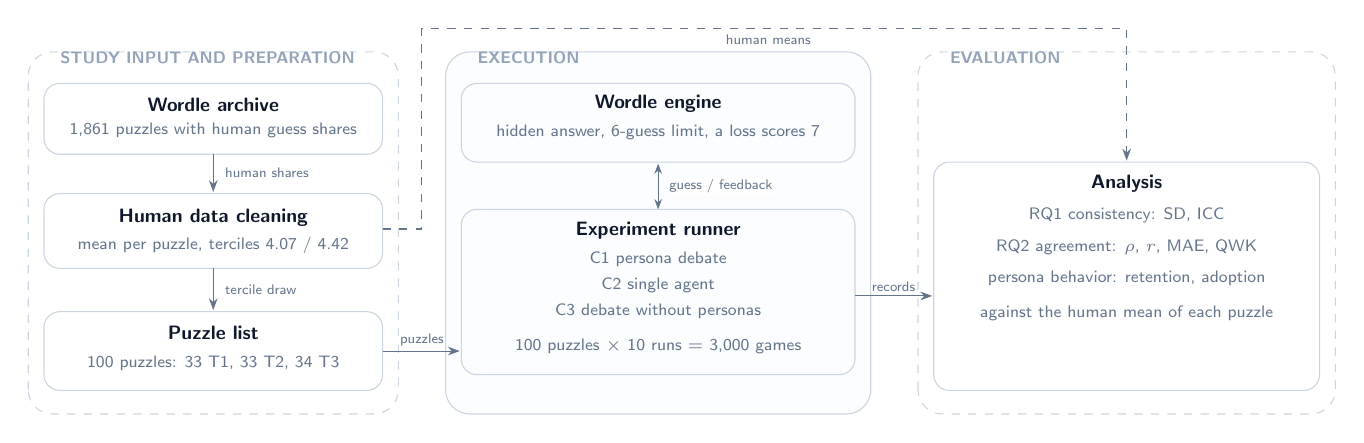
\begin{tikzpicture}[x=1cm,y=1cm,line width=0.4pt]

% ---------- containers ----------
\draw[rounded corners=3.1mm, dashed, line] (0.20,2.00) rectangle (4.90,6.60);
\draw[rounded corners=3.1mm, line, fill=panel] (5.50,2.00) rectangle (10.90,6.60);
\draw[rounded corners=3.1mm, dashed, line] (11.50,2.00) rectangle (16.80,6.60);
\node[anchor=south west, inner sep=0] at (0.60,6.44) {\panellabel{STUDY INPUT AND PREPARATION}};
\node[anchor=south west, inner sep=0] at (5.90,6.44) {\panellabel{EXECUTION}};
\node[anchor=south west, inner sep=0] at (11.90,6.44) {\panellabel{EVALUATION}};

% ---------- input ----------
\draw[rounded corners=2mm, line] (0.40,5.30) rectangle (4.70,6.20);
\node[anchor=center, inner sep=0] at (2.55,5.93) {\cardtitle{Wordle archive}};
\node[anchor=center, inner sep=0] at (2.55,5.60) {\cardsub{1,861 puzzles with human guess shares}};

\draw[rounded corners=2mm, line] (0.40,3.85) rectangle (4.70,4.80);
\node[anchor=center, inner sep=0] at (2.55,4.50) {\cardtitle{Human data cleaning}};
\node[anchor=center, inner sep=0] at (2.55,4.14) {\cardsub{mean per puzzle, terciles 4.07 / 4.42}};

\draw[rounded corners=2mm, line] (0.40,2.30) rectangle (4.70,3.30);
\node[anchor=center, inner sep=0] at (2.55,3.03) {\cardtitle{Puzzle list}};
\node[anchor=center, inner sep=0] at (2.55,2.64) {\cardsub{100 puzzles: 33 T1, 33 T2, 34 T3}};

% ---------- execution ----------
\draw[rounded corners=2mm, line] (5.70,5.20) rectangle (10.70,6.20);
\node[anchor=center, inner sep=0] at (8.20,5.94) {\cardtitle{Wordle engine}};
\node[anchor=center, inner sep=0] at (8.20,5.58) {\cardsub{hidden answer, 6-guess limit, a loss scores 7}};

\draw[rounded corners=2mm, line] (5.70,2.50) rectangle (10.70,4.60);
\node[anchor=center, inner sep=0] at (8.20,4.33) {\cardtitle{Experiment runner}};
\node[anchor=center, inner sep=0] at (8.20,3.96) {\cardsub{C1 persona debate}};
\node[anchor=center, inner sep=0] at (8.20,3.63) {\cardsub{C2 single agent}};
\node[anchor=center, inner sep=0] at (8.20,3.30) {\cardsub{C3 debate without personas}};
\node[anchor=center, inner sep=0] at (8.20,2.86) {\cardsub{100 puzzles $\times$ 10 runs $=$ 3,000 games}};

% ---------- evaluation ----------
\draw[rounded corners=2mm, line] (11.70,2.30) rectangle (16.60,5.20);
\node[anchor=center, inner sep=0] at (14.15,4.92) {\cardtitle{Analysis}};
\node[anchor=center, inner sep=0] at (14.15,4.52) {\cardsub{RQ1 consistency: SD, ICC}};
\node[anchor=center, inner sep=0] at (14.15,4.12) {\cardsub{RQ2 agreement: $\rho$, $r$, MAE, QWK}};
\node[anchor=center, inner sep=0] at (14.15,3.72) {\cardsub{persona behavior: retention, adoption}};
\node[anchor=center, inner sep=0] at (14.15,3.28) {\cardsub{against the human mean of each puzzle}};

% ---------- arrows ----------
\draw[-{Stealth[length=1.5mm,width=1.1mm]}, draw=muted] (2.55,5.30) -- (2.55,4.82);
\node[anchor=west, inner sep=0.4pt, fill=white] at (2.68,5.06) {\plabel{human shares}};

\draw[-{Stealth[length=1.5mm,width=1.1mm]}, draw=muted] (2.55,3.85) -- (2.55,3.32);
\node[anchor=west, inner sep=0.4pt, fill=white] at (2.68,3.58) {\plabel{tercile draw}};

\draw[-{Stealth[length=1.5mm,width=1.1mm]}, draw=muted] (4.70,2.80) -- (5.68,2.80);
\node[anchor=south, inner sep=0.4pt, fill=white] at (5.20,2.84) {\plabel{puzzles}};

\draw[{Stealth[length=1.3mm]}-{Stealth[length=1.3mm]}, draw=muted, line width=0.45pt] (8.20,4.60) -- (8.20,5.18);
\node[anchor=west, inner sep=0.4pt, fill=white] at (8.32,4.89) {\plabel{guess / feedback}};

\draw[-{Stealth[length=1.5mm,width=1.1mm]}, draw=muted] (10.70,3.50) -- (11.68,3.50);
\node[anchor=south, inner sep=0.4pt, fill=white] at (11.19,3.54) {\plabel{records}};

% human baseline route: right of the input panel, over the top, down into the analysis
\draw[-{Stealth[length=1.5mm,width=1.1mm]}, draw=muted, dashed]
  (4.70,4.35) -- (5.20,4.35) -- (5.20,6.90) -- (14.15,6.90) -- (14.15,5.22);
\node[anchor=north, inner sep=0.4pt, fill=white] at (9.60,6.84) {\plabel{human means}};

\end{tikzpicture}
\end{document}
